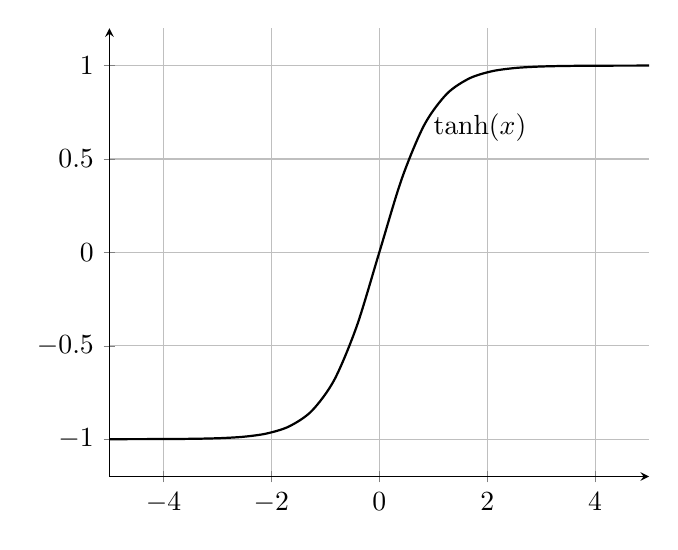
\begin{tikzpicture}
    \begin{axis}[
        % xlabel = $x$,
        % ylabel = $\tanh{x}$,
        ymin = -1.2,ymax = 1.2,
        domain = -6:6,
        grid=both,
        % width=5.5cm,
        smooth,
        axis lines = left,
    ]
  
    \addplot[color=black,domain=-5:5,thick]{(1-exp(-2*x))/(1+exp(-2*x))} node[pos=0.6,anchor=west]{$\tanh(x)$};
    %   \addplot[color=blue]{tanh(x)};
    %   \addplot[color=blue,dashed,domain=-1:1,thin]{x};
    \end{axis}
    % \draw (0,-1) node [inner sep=0.75pt]{
    %   $\sigmoid{x} =\frac{1}{1+e^{-x}}$
    % };
\end{tikzpicture}
